\input{preamble.tex}

\title{Observability Data Engineering}
\subtitle{A Story About Math, Four Golden Signals, and Business Intelligence}
\institute{DevOps Observability Architect}
\author{Jack Neely\\ jjneely@gmail.com}

\date{\today}

\tikzstyle{process} = [
    rectangle,
    minimum width=2.5cm, 
    minimum height=0.75cm,
    text centered, 
    draw=black, 
    fill=white,
]
\tikzstyle{textstyle} = [
    rectangle,
    align=left,
    minimum width=1.5cm, 
    minimum height=0.75cm,
]
\tikzstyle{arrow} = [
    thick,
    ->,
    >=stealth
]

\begin{document}

\begin{frame}[fragile]
    \centering
    \resizebox{\textwidth}{!}{%
    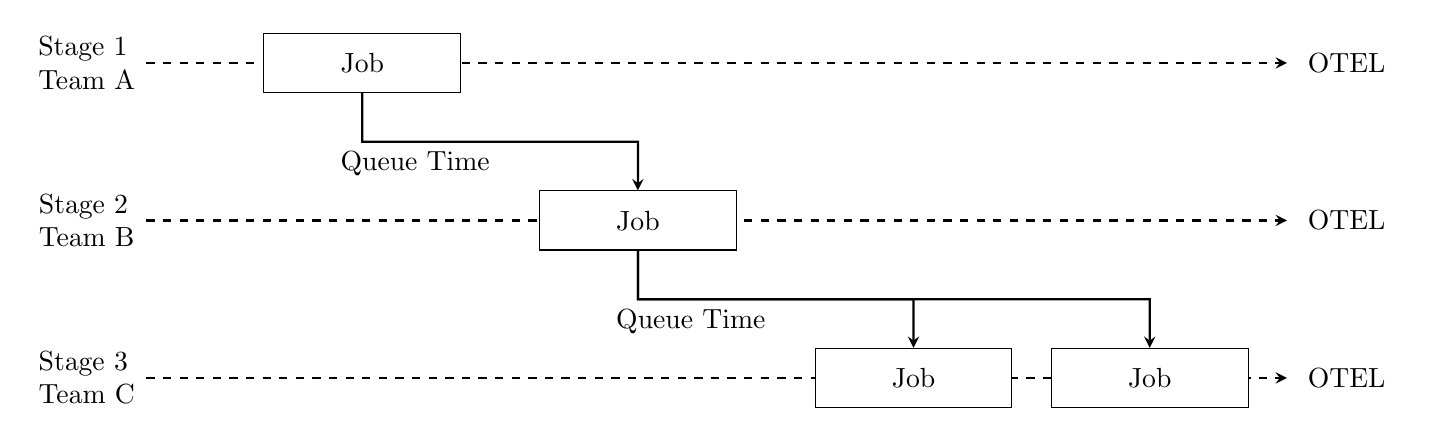
\begin{tikzpicture}[node distance=2cm]
        %%\draw[step=1cm,gray,very thin] (0,0) grid (15,-10);
        \node (stage1) [textstyle] {Stage 1\\Team A};
        \node (stage2) [textstyle, below of=stage1] {Stage 2\\Team B};
        \node (stage3) [textstyle, below of=stage2] {Stage 3\\Team C};
        \node (otel1) [textstyle, right of=stage1, xshift=14cm] {OTEL};
        \node (otel2) [textstyle, right of=stage2, xshift=14cm] {OTEL};
        \node (otel3) [textstyle, right of=stage3, xshift=14cm] {OTEL};
        \draw [arrow,dashed] (stage1) -- (otel1);
        \draw [arrow,dashed] (stage2) -- (otel2);
        \draw [arrow,dashed] (stage3) -- (otel3);
        \node (job1) [process, right of=stage1, xshift=1.5cm] {Job};
        \node (job2) [process, right of=stage2, xshift=5cm] {Job};
        \node (job3) [process, right of=stage3, xshift=8.5cm] {Job};
        \node (job4) [process, right of=job3, xshift=1cm] {Job};
        \draw [arrow] (job1) -- (3.5,-1) -- node[anchor=north east] {Queue Time} (7,-1) -- (job2);
        \draw [arrow] (job2) -- (7, -3) -- node[anchor=north east] {Queue Time} (10.5, -3) -- (job3);
        \draw [arrow] (job2) -- (7, -3) -- (13.5, -3) -- (job4);
    \end{tikzpicture}}
\end{frame}

\end{document}
